%%%%%%%%%%%%%%%%%%%%%%%%%%%%%%%%%%%%%%%%%%%%%%%%%%%%%%%%%%%%%%%%%%
\section{Numerical model}
\label{sec:numericalmodel}
%%%%%%%%%%%%%%%%%%%%%%%%%%%%%%%%%%%%%%%%%%%%%%%%%%%%%%%%%%%%%%%%%%

%%%%%%%%%%%%%%%%%%%%%%%%%%%%%%%%%%%%%%%%%%%%%%%%%%%%%%%%%%%%%%%%%%
\subsection{Finite volume discretisation of the beam}
\label{sec:beamFVDiscretisation}
%%%%%%%%%%%%%%%%%%%%%%%%%%%%%%%%%%%%%%%%%%%%%%%%%%%%%%%%%%%%%%%%%%

\noindent
The beam domain $s\in[0,L]$ is discretised into non-overlapping one-dimensional control volumes (CVs). The centreline position and the rotation parameters are stored at the CV centres, the spatial resultants $(\mathbf{n},\mathbf{m})$ are evaluated at the faces by linear interpolation of the cell-centred kinematic quantities, and the external loading is collocated at the cell centre \citep{bali_cell-centered_2022}. Integrating Eqs.~\eqref{eq:ForceBalanceDynamic}--\eqref{eq:MomentBalanceDynamic} over a cell $P$ of length $L_{P}$, bounded by the faces $w$ and $e$ and neighboured by the cells $W$ and $E$, gives the locally conservative discrete form
\begin{align}
\mathbf{n}_{e} - \mathbf{n}_{w} + \mathbf{f}_{P}\,L_{P} &= \rho_{b}A\,L_{P}\,\ddot{\mathbf{w}}_{P}, \label{eq:fvForceBalance} \\
\mathbf{m}_{e} - \mathbf{m}_{w} + \bigl(\mathbf{r}'\times\mathbf{n}\bigr)_{P}\,L_{P} + \mathbf{t}_{P}\,L_{P} &= L_{P}\,\boldsymbol{\Lambda}_{P}\bigl(\mathbf{I}_{\rho}\dot{\boldsymbol{\Omega}}_{P} + \boldsymbol{\Omega}_{P}\times(\mathbf{I}_{\rho}\boldsymbol{\Omega}_{P})\bigr), \label{eq:fvMomentBalance}
\end{align}
with the cell-centre source terms already using the midpoint-rule approximation of the volume integral. The face resultants are nonlinear functions of the kinematic unknowns at cells $P$, $W$, and $E$.

\noindent
The unknowns at each CV centre are organised as the six-component increment $\boldsymbol{\phi}_P = (\Delta\mathbf{w}_P,\,\Delta\boldsymbol{\psi}_P)^{T}$ between successive Newton iterates, so the translational and rotational rows are solved simultaneously. Linearising about the current iterate gives the three-point finite volume form
\begin{equation}
\mathbf{A}_{W}\,\boldsymbol{\phi}_{W} \;+\; \mathbf{A}_{P}\,\boldsymbol{\phi}_{P} \;+\; \mathbf{A}_{E}\,\boldsymbol{\phi}_{E} \;=\; \mathbf{b}_{P},
\label{eq:fvDiscreteSystem}
\end{equation}
in which the coefficients are dense $6\times 6$ blocks mixing the translation and rotation rows, which the moment-balance cross-product $\mathbf{r}'\times\mathbf{n}$ couples tightly, and $\mathbf{b}_{P}$ is the residual of cell $P$. Assembling over all CVs yields a sparse block-tridiagonal system of size $6N_b\times 6N_b$, where $N_b$ is the number of beam cells. It is solved by a Newton--Raphson iteration in which the kinematic fields are updated cell by cell,
\begin{equation}
\mathbf{w}^{(k+1)} \;=\; \mathbf{w}^{(k)} + \Delta\mathbf{w}^{(k)},
\qquad
\boldsymbol{\Lambda}^{(k+1)} \;=\; \exp\!\left(\widehat{\Delta\boldsymbol{\psi}^{(k)}}\right)\,\boldsymbol{\Lambda}^{(k)},
\label{eq:beamNewtonUpdate}
\end{equation}
until both the increment norm and the residual norm fall below prescribed tolerances. The tangent coefficients and the verification of the discretisation are given by \citet{bali_cell-centered_2022,bali_finite_2024}, and its OpenFOAM implementation by \citet{bali_beamfoam_2025}. All transient results reported here integrate the acceleration terms with a first-order backward scheme, in which the current-level unknown appears linearly, so the inertia term contributes a diagonal-block coefficient of $\rho_{b}A\,L_{P}/\Delta t^{2}$ to $\mathbf{A}_{P}$, the history terms enter the residual, and the block-tridiagonal structure is unchanged. Time steps between $10^{2}$ and $4\times10^{4}$ steps per forcing period are used, and each transient case is started from rest.

%%%%%%%%%%%%%%%%%%%%%%%%%%%%%%%%%%%%%%%%%%%%%%%%%%%%%%%%%%%%%%%%%%
\subsection{Actuator-line beam--fluid coupling}
\label{sec:almCouplingTheory}
%%%%%%%%%%%%%%%%%%%%%%%%%%%%%%%%%%%%%%%%%%%%%%%%%%%%%%%%%%%%%%%%%%

\noindent
The beam centreline carries a set of \emph{actuator points} $\mathbf{P}_{a,i}$, one per beam control volume, at which the kinematic state of the beam is sampled and the hydrodynamic interaction is concentrated. Each actuator point follows the beam-cell centre as the structure deforms, the surrounding Eulerian mesh remains stationary, and the hydrodynamic exchange is realised through the volumetric source $\mathbf{S}_{m}$ of Eq.~\eqref{eq:momentum}. The strategy follows the centreline-forcing approach of \citet{bral_development_2025,bral_modeling_2025}, and extends it in two ways. The structural side is the cell-centred finite volume beam of Section~\ref{sec:beamFVDiscretisation} rather than a finite element discretisation, so the beam unknowns reside on the same data structures as the fluid unknowns and are updated within the same outer time loop, and the sampling and projection operators are implemented in a parallel-consistent form that scales to domain-decomposed fluid meshes (Section~\ref{sec:almParallelSearch}).

\noindent
Two transfer operations are needed at each time step. The first samples the local fluid velocity near each actuator point and uses it to evaluate the hydrodynamic line force on the beam. The second projects the equal and opposite reaction back onto the fluid mesh as a regularised volumetric source. They are treated differently by design. Velocity sampling is confined to a single fluid cell per beam cell to avoid contamination from the modified flow induced by the source itself, whereas force projection is smoothed over neighbouring cells through a Gaussian kernel, because a singular line force cannot be imposed on a discretisation of finite resolution without severe grid dependence.

\subsubsection{Centreline coupling conditions}
In body-fitted FSI the kinematic and dynamic coupling conditions are imposed at a resolved fluid--solid surface, where velocities match and tractions are equal and opposite. The centreline formulation replaces this surface exchange with two transfer operations on the actuator points. Kinematically, each actuator point tracks the position and velocity of its beam cell,
\begin{equation}
\mathbf{P}_{a,i}(t) \;=\; \mathbf{P}_{a,i}^{\,0} + \mathbf{W}_{i}(t),
\qquad
\dot{\mathbf{P}}_{a,i}(t) \;=\; \mathbf{U}_{b,i}(t),
\label{eq:almKinematicCoupling}
\end{equation}
where $\mathbf{P}_{a,i}^{\,0}$ is the initial position, $\mathbf{W}_{i}$ the translational displacement of beam cell $i$, and $\mathbf{U}_{b,i}$ the beam-cell velocity. No no-slip condition is imposed, because the beam surface is not represented in the fluid mesh. The rotation field enters only implicitly, through the local tangent used to decompose the relative velocity. Dynamically, the sampled relative velocity gives a line force $\mathbf{f}_{i}$ per unit beam length acting on the beam, and the fluid receives the equal and opposite force distributed as a regularised source, so the discrete coupling satisfies the action--reaction condition in integral form,
\begin{equation}
\sum_{i} \mathbf{f}_{i}\,L_{i} \;+\; \sum_{j} \mathbf{S}_{m,j}\,V_{j} \;\approx\; \mathbf{0},
\label{eq:almActionReaction}
\end{equation}
with $L_{i}$ the beam-cell length and $V_{j}$ the volume of fluid cell $j$.

\noindent
Equation~\eqref{eq:almActionReaction} is a statement about the transferred load alone, and not a momentum balance over a region of material. Each subsystem carries its own inertia in its own momentum equation, and those terms are untouched by the exchange, so the relation plays the same role as the equality of tractions across a resolved interface in body-fitted FSI, where the interface itself carries no mass. For the \emph{resultant} force the exchange is conservative, because the normalisation of Section~\ref{sec:almProjection} rescales the projected source so that its discrete volume integral matches the force carried by the actuator segments. What remains approximate is the spatial distribution. The kernel spreads the reaction over a finite region rather than along the centreline, so the moment of the applied source about a given point differs from that of the line load by an amount that scales with the kernel width, and the angular-momentum transfer differs with it.

\noindent
Figure~\ref{fig:almCouplingSchematic} summarises the information exchange between the three components.

\begin{figure}[!ht]
\centering
\resizebox{0.80\textwidth}{!}{%
\begin{tikzpicture}[x=1cm,y=1cm,>=Latex,font=\normalsize]
  \tikzstyle{block}=[draw,rounded corners=3pt,minimum width=7.5cm,minimum height=1.55cm,align=center,very thick]
  \tikzstyle{steplabel}=[draw,circle,thick,fill=white,inner sep=0.5pt,minimum size=0.62cm,font=\small\bfseries]

  % three main blocks vertically stacked
  \node[block,fill=blue!8]    (fluid) at (0, 4.0) {\textbf{Fluid finite volume solver}\\Eulerian mesh, Eqs.~(\ref{eq:continuity})--(\ref{eq:momentum})};
  \node[block,fill=gray!10]   (alm)   at (0, 0.0) {\textbf{Actuator-line coupling operator}\\velocity sampling and force projection};
  \node[block,fill=orange!10] (beam)  at (0,-4.0) {\textbf{Finite volume Simo--Reissner beam solver}\\centreline mesh, Eqs.~(\ref{eq:fvForceBalance})--(\ref{eq:fvMomentBalance})};

  % --- vertical arrows between fluid and alm ---
  \draw[->,very thick,blue!70!black]
       ([xshift=-1.3cm]fluid.south) -- ([xshift=-1.3cm]alm.north)
       node[midway,left,font=\small,align=right]
       {sampled fluid velocity\\$\mathbf{U}_{c(\mathbf{P}_{s,i})}$};
  \node[steplabel] at (-1.3, 3.0) {3};
  \draw[->,very thick,red!75!black]
       ([xshift=1.3cm]alm.north) -- ([xshift=1.3cm]fluid.south)
       node[midway,right,font=\small,align=left]
       {reaction source\\$\mathbf{S}_{m,j}$};
  \node[steplabel] at (1.3, 1.0) {4};

  % --- vertical arrows between beam and alm ---
  \draw[->,very thick,orange!80!black]
       ([xshift=-1.3cm]beam.north) -- ([xshift=-1.3cm]alm.south)
       node[midway,left,font=\small,align=right]
       {actuator-point kinematics\\$\mathbf{P}_{a,i},\;\dot{\mathbf{P}}_{a,i}$};
  \node[steplabel] at (-1.3,-3.0) {2};
  \draw[->,very thick,purple!80!black]
       ([xshift=1.3cm]alm.south) -- ([xshift=1.3cm]beam.north)
       node[midway,right,font=\small,align=left]
       {line load\\$\mathbf{f}_{i}\,L_{i}$};
  \node[steplabel] at (1.3,-1.0) {5};

  \node[draw,thick,fill=yellow!25,rounded corners=2pt,
        minimum width=2.8cm,minimum height=0.75cm,font=\small,align=center]
       (start) at (-7.0,-4.0) {\textbf{start of}\\\textbf{time step}};
  \draw[->,very thick,black] (start.east) -- (beam.west);
  \node[steplabel] at (-5.0,-4.0) {1};

  \node[draw,thick,fill=yellow!25,rounded corners=2pt,
        minimum width=2.8cm,minimum height=0.75cm,font=\small,align=center]
       (next) at ( 7.0, 4.0) {\textbf{next}\\\textbf{time step}};
  \draw[->,very thick,black] (fluid.east) -- (next.west);
  \node[steplabel] at ( 5.0, 4.0) {6};
\end{tikzpicture}
}
\caption{Centreline coupling drawn as a per-time-step data-flow diagram between the three solver components. \protect\textcircled{1} The beam solver advances the structural state and produces the current actuator-point positions and velocities; \protect\textcircled{2} these pass to the coupling operator; \protect\textcircled{3} the fluid solver supplies the upstream-sampled velocity at every actuator point; the operator evaluates the hydrodynamic line force and returns it as \protect\textcircled{4} a regularised volumetric reaction source to the fluid solver and \protect\textcircled{5} an equal and opposite line load to the beam solver; \protect\textcircled{6} the fluid pressure--velocity system is advanced before the next time step. The sequence runs once per time step, on the first outer iteration of the PIMPLE loop, so the reaction source of \protect\textcircled{4} stays fixed for the remaining outer iterations.}
\label{fig:almCouplingSchematic}
\end{figure}

\subsubsection{Actuator points and velocity sampling}
\label{sec:almSampling}
The actuator-point position is reconstructed from three quantities stored on the beam mesh,
\begin{equation}
\mathbf{P}_{a,i}
\;=\;
\mathbf{C}^{b}_{i}
\;+\;
\mathbf{W}^{\mathrm{ref}}_{i}
\;+\;
\mathbf{W}_{i},
\label{eq:almActuatorPoint}
\end{equation}
where $\mathbf{C}^{b}_{i}$ is the initial beam-cell centre, $\mathbf{W}^{\mathrm{ref}}_{i}$ a fixed offset that places the actuator point at a chosen material location relative to the cell centre (typically zero, but retained so the point can be shifted onto, for example, the upper surface of a non-axisymmetric cross-section), and $\mathbf{W}_{i}$ the current displacement. The actuator-point velocity is the time derivative of Eq.~\eqref{eq:almActuatorPoint} and equals the beam-cell translational velocity, because the first two terms are time-independent. The local tangent $\mathbf{e}_{t,i}$ is reconstructed from a Hermite spline through the current beam-cell centres, and is needed both to decompose the relative velocity and to define the upstream sampling direction.

\noindent
The sampling point is placed at a fixed distance upstream of the actuator point, in a direction reconstructed locally from the incoming flow, as Figure~\ref{fig:almSamplingSchematic} shows. A preliminary relative velocity is first evaluated at the actuator point itself,
\begin{equation}
\mathbf{u}^{0}_{r,i}
\;=\;
\mathbf{U}_{c(\mathbf{P}_{a,i})}
\;-\;
\dot{\mathbf{P}}_{a,i},
\label{eq:almPreliminaryVelocity}
\end{equation}
where $\mathbf{U}_{c(\mathbf{P}_{a,i})}$ is the velocity stored in the single fluid cell containing $\mathbf{P}_{a,i}$ and $c(\cdot)$ denotes the point-to-cell search operator. This value is used only to orient the sampling stencil, not as the line-force velocity, because the modified flow induced by the source near the beam would contaminate the force estimate. Its component normal to the beam tangent, $\mathbf{u}^{0}_{n,i} = \mathbf{u}^{0}_{r,i} - (\mathbf{u}^{0}_{r,i}\!\cdot\!\mathbf{e}_{t,i})\mathbf{e}_{t,i}$, fixes the upstream direction $\mathbf{e}_{s,i} = -\mathbf{u}^{0}_{n,i}/\lVert\mathbf{u}^{0}_{n,i}\rVert$, and the sampling point follows as
\begin{equation}
\mathbf{P}_{s,i}
\;=\;
\mathbf{P}_{a,i}
\;+\;
\bigl[\mathbf{I} - \mathbf{n}_{p}\mathbf{n}_{p}^{T}\bigr]\,\ell_{s}\,\mathbf{e}_{s,i},
\label{eq:almSamplingPoint}
\end{equation}
where $\ell_{s}$ is the sampling distance and $\mathbf{n}_{p}$ a prescribed plane normal used to flatten the stencil onto a chosen plane in three-dimensional simulations. When $\lVert\mathbf{u}^{0}_{n,i}\rVert$ falls below a small threshold, for example because the beam is nearly aligned with the flow or the flow has stagnated, the unit vector becomes ill-conditioned and the implementation switches to a fallback direction, namely the user-prescribed global upstream direction projected onto the local cross-section plane and renormalised. Because the projector in Eq.~\eqref{eq:almSamplingPoint} removes the component of $\mathbf{e}_{s,i}$ along $\mathbf{n}_{p}$ without renormalising, the realised offset is bounded above by $\ell_{s}$ and equals it only when $\mathbf{e}_{s,i}$ already lies in the sampling plane, which holds in every configuration studied here. The distance itself is set as $\ell_{s} = r_{s}^{\star}L_{\mathrm{ref}}$, with $L_{\mathrm{ref}}$ the beam radius for circular cross-sections and a representative cross-section dimension otherwise, so its dimensional value is problem-dependent rather than universal. Its influence on the response is examined directly in Section~\ref{sec:beamtunnel_sensitivity}.

\noindent
Once the sampling point has been located, the fluid cell containing it is found by the same operator, and the velocity stored in that single cell defines the relative velocity used by the line-force model,
\begin{equation}
\mathbf{U}_{r,i}
\;=\;
\mathbf{U}_{c(\mathbf{P}_{s,i})}
\;-\;
\dot{\mathbf{P}}_{a,i}.
\label{eq:almRelativeVelocity}
\end{equation}
No averaging across neighbouring cells is performed. This is a deliberate simplification compared with integral or line-averaged sampling, which removes the dependence on a sampling-volume definition and keeps the sampling local, and which avoids using the velocity at the actuator point itself, where the regularised source slows the flow and would bias the drag estimate downward.

\begin{figure}[!ht]
\centering
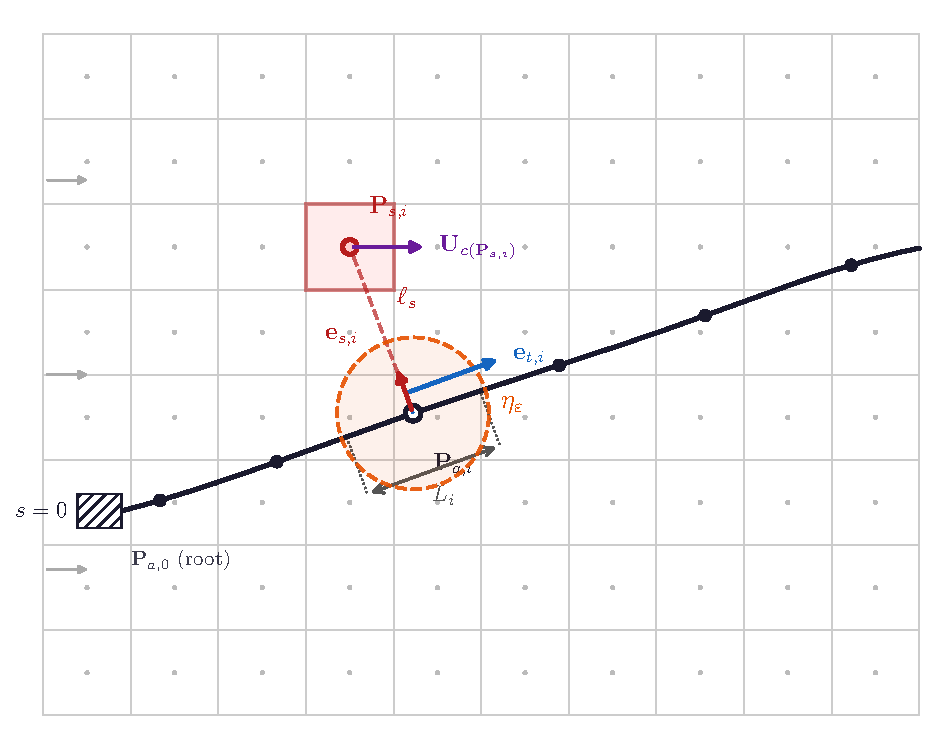
\includegraphics[width=0.92\textwidth]{alm_sampling.pdf}
\caption{Actuator-line velocity sampling. The beam cell centre defines the actuator point $\mathbf{P}_{a,i}$; the tangent $\mathbf{e}_{t,i}$ and upstream direction $\mathbf{e}_{s,i}$ locate the sampling point $\mathbf{P}_{s,i}$ at distance $\ell_s$. The highlighted CFD cell supplies the sampled velocity, and the dashed circle indicates the Gaussian regularisation support $\eta_{\varepsilon}$ used for the reaction force projection. The uniform square grid is used for illustration only, and the procedure applies unchanged to unstructured meshes of general polyhedral cells.}
\label{fig:almSamplingSchematic}
\end{figure}

\subsubsection{Line-force evaluation}
\label{sec:almLineForce}
The relative velocity of Eq.~\eqref{eq:almRelativeVelocity} is split into a tangential component $\mathbf{U}_{t,i} = (\mathbf{U}_{r,i}\!\cdot\!\mathbf{e}_{t,i})\mathbf{e}_{t,i}$, which controls the skin-friction contribution, and a normal component $\mathbf{U}_{n,i} = \mathbf{U}_{r,i} - \mathbf{U}_{t,i}$, which controls the cross-flow drag that dominates for slender bluff bodies. The two are combined into the quasi-steady line force per unit beam length,
\begin{equation}
\mathbf{f}^{*}_{i}
\;=\;
-\,\tfrac{1}{2}\,\rho_{f}\,d\,
\bigl\lVert\mathbf{U}_{r,i}\bigr\rVert
\bigl(C_{dn}\mathbf{U}_{n,i} + C_{dt}\mathbf{U}_{t,i}\bigr),
\label{eq:almLineForce}
\end{equation}
which is the discrete form of Eq.~\eqref{eq:fext_drag}, with the negative sign ensuring that the force opposes the relative motion of the fluid with respect to the beam. The raw value is sensitive to small fluctuations of the sampled velocity between successive coupling updates, which can excite spurious oscillations in the structural response, so a first-order relaxation against the value from the previous coupling update stabilises the coupling,
\begin{equation}
\mathbf{f}_{i}
\;=\;
\alpha_{f}\,\mathbf{f}^{*}_{i}
\;+\;
(1 - \alpha_{f})\,\mathbf{f}^{\,\mathrm{prev}}_{i},
\label{eq:almForceRelaxation}
\end{equation}
with $\alpha_{f}\in(0,1]$ set to unity to recover the un-relaxed update. Because the line force is evaluated once per time step (Section~\ref{sec:almParallelSearch}), $\mathbf{f}^{\,\mathrm{prev}}_{i}$ is the relaxed force of the previous time step. On the beam side the relaxed value is multiplied by the cell length before being added to the structural residual of Eq.~\eqref{eq:fvForceBalance}, and on the fluid side it enters the regularised source with the opposite sign.

\subsubsection{Projection to the fluid mesh}
\label{sec:almProjection}
Only the fluid cells near the actuator line take part in the projection. A cell whose centre $\mathbf{C}_{j}$ lies outside the bounding box of the actuator points, inflated by $3\varepsilon$ in every direction, is skipped before any distance is evaluated. For the remaining cells, the closest actuator segment is identified by evaluating the distance from $\mathbf{C}_{j}$ to each segment of the actuator line, and the cost of this step is discussed in Section~\ref{sec:almParallelSearch}. If the closest segment lies between $\mathbf{P}_{a,i}$ and $\mathbf{P}_{a,i+1}$, the foot of the perpendicular from $\mathbf{C}_{j}$ onto the segment defines the projection point
\begin{equation}
\mathbf{P}_{\parallel,j}
\;=\;
(1-s_{j})\,\mathbf{P}_{a,i} \;+\; s_{j}\,\mathbf{P}_{a,i+1},
\qquad
0\le s_{j}\le 1,
\label{eq:almProjectionPoint}
\end{equation}
and the radial distance to the segment is $r_{j} = \lVert\mathbf{C}_{j} - \mathbf{P}_{\parallel,j}\rVert$. The line force is spread over the surrounding cells with a two-dimensional Gaussian kernel,
\begin{equation}
\eta_{\varepsilon}(r_{j})
\;=\;
\frac{1}{\pi\varepsilon^{2}}\exp\!\left[-\!\left(\frac{r_{j}}{\varepsilon}\right)^{\!2}\right],
\label{eq:almGaussian}
\end{equation}
where $\varepsilon$ is the regularisation width, whose influence is examined in Section~\ref{sec:beamtunnel_sensitivity}. The kernel is truncated at $r_{j} = 3\varepsilon$, so cells farther than $3\varepsilon$ from the actuator line receive no source. The part of the kernel discarded by this truncation is a fraction $e^{-9} \approx 1.2\times10^{-4}$ of its integral, and the normalisation below returns it to the retained cells, so the truncation does not change the transferred force. The geometry of the projection is illustrated in Figure~\ref{fig:almProjectionSchematic}.

\begin{figure}[!ht]
\centering
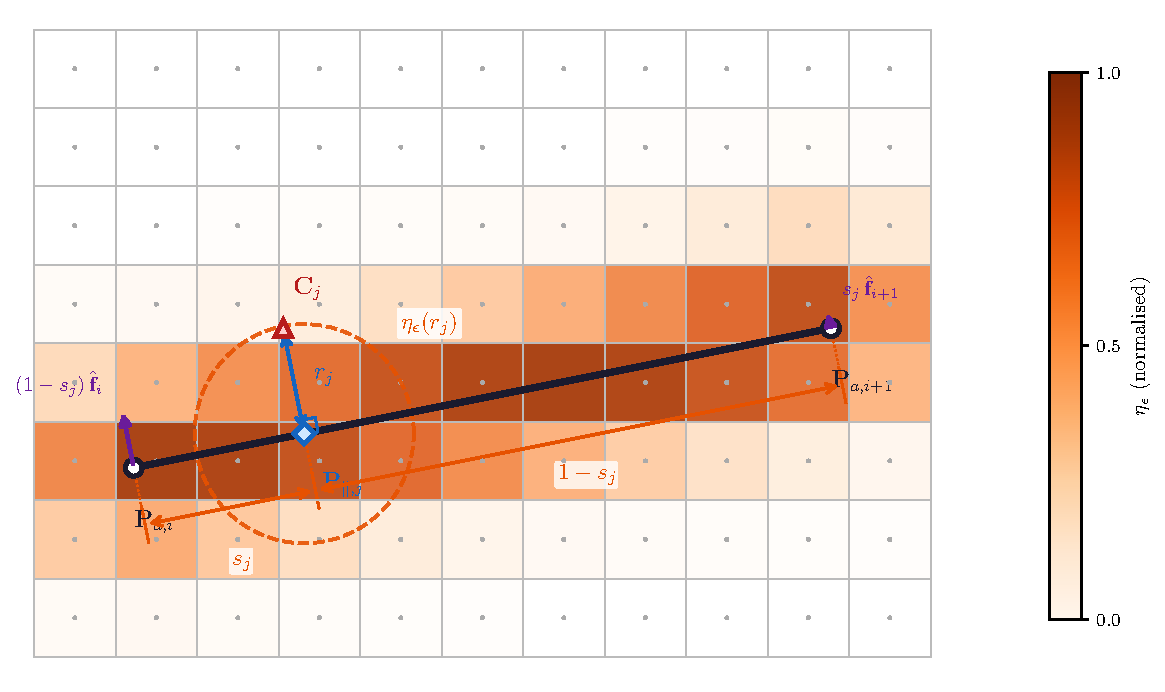
\includegraphics[width=0.90\textwidth]{alm_projection.pdf}
\caption{Regularised force projection from an actuator segment to the fluid mesh. The CFD cells are coloured by the normalised Gaussian weight $\eta_{\varepsilon}$ centred on the projection point $\mathbf{P}_{\parallel,j}$. The source contribution to cell $j$ comes from linear interpolation of the normalised nodal forces along the segment, weighted by $\eta_{\varepsilon}(r_j)$. As in Figure~\ref{fig:almSamplingSchematic}, the uniform grid is for illustration only.}
\label{fig:almProjectionSchematic}
\end{figure}

\noindent
The projected force is normalised so that the volume integral of the applied source is consistent with the force carried by the beam segment. For beam point $k$ the weight is accumulated as $w_k = \sum_{j}\omega_{jk}\eta_{\varepsilon}(r_j)V_j$, where $V_j$ is the fluid-cell volume and $\omega_{jk}$ the linear interpolation weight, with $\omega_{ji}=1-s_j$ and $\omega_{j,i+1}=s_j$. The normalised nodal force is $\widehat{\mathbf{f}}_k = \mathbf{f}_k\Delta s_k / w_k$, with $\Delta s_k$ the local actuator-segment length, and the source applied to a fluid cell is
\begin{equation}
\mathbf{S}_{m,j}^{(i)}
=
-\eta_{\varepsilon}(r_j)
\left[
(1-s_j)\widehat{\mathbf{f}}_{i}
+
s_j\widehat{\mathbf{f}}_{i+1}
\right],
\label{eq:almMomentumSource}
\end{equation}
the negative sign indicating that the source is the reaction applied to the fluid. It is integrated over the receiving cell with the cell-centred midpoint rule, consistent with the second-order accuracy of the surrounding finite volume operators.

\noindent
This normalisation conserves the resultant force by construction. Summing Eq.~\eqref{eq:almMomentumSource} over all fluid cells and regrouping by beam point gives $\sum_{j}\mathbf{S}_{m,j}V_{j} = -\sum_{k}\widehat{\mathbf{f}}_{k}\,w_{k} = -\sum_{k}\mathbf{f}_{k}\,\Delta s_{k}$, so the total force applied to the fluid equals the total actuator-line load, whatever the mesh, kernel width, or kernel truncation, provided every accumulated weight is non-zero. Without the normalisation, the discrete volume integral of the kernel differs from its continuous value whenever the kernel is under-resolved by the mesh or truncated, and the force applied to the fluid then differs from the load carried by the beam. That condition holds whenever at least one fluid cell is assigned to each actuator segment. The same guarantee does not extend to angular momentum, since the kernel redistributes the force away from the centreline.

\subsubsection{Coupled update sequence and parallel-consistent search}
\label{sec:almParallelSearch}
Algorithm~\ref{alg:almCoupling} summarises the operations performed within one time step and shows where the coupling sits inside the PIMPLE loop. Each operation is labelled with the equation it implements.

\begin{algorithm}[!ht]
\caption{Actuator-line beam--fluid coupling within one time step. The coupling operations of steps~\ref{alg:stepActuator}--\ref{alg:stepSource} run only on the first outer iteration of the PIMPLE loop, and the source $\mathbf{S}_{m,j}$ they produce is held fixed for the remaining outer iterations.}
\label{alg:almCoupling}
\begin{algorithmic}[1]
\FOR{each time step, from $t^{n}$ to $t^{n+1}$}
\FOR{each PIMPLE outer iteration $k = 1,\ldots,n_{\mathrm{out}}$}
\IF{$k = 1$}
\STATE Evaluate the actuator-point positions $\mathbf{P}_{a,i}$ and velocities $\dot{\mathbf{P}}_{a,i}$ of all beam cells $i=1,\ldots,N_{b}$ from the beam state at $t^{n}$, using Eqs.~\eqref{eq:almKinematicCoupling} and~\eqref{eq:almActuatorPoint}, and the centreline tangents $\mathbf{e}_{t,i}$. \label{alg:stepActuator}
\STATE Locate the fluid cell containing each actuator point and evaluate the preliminary relative velocity $\mathbf{u}^{0}_{r,i}$ from Eq.~\eqref{eq:almPreliminaryVelocity}. \label{alg:stepLocateA}
\STATE Construct the upstream sampling points $\mathbf{P}_{s,i}$ from Eq.~\eqref{eq:almSamplingPoint}, with the fallback direction triggered when $\lVert\mathbf{u}^{0}_{n,i}\rVert$ falls below the prescribed threshold. \label{alg:stepSamplingPts}
\STATE Locate the single fluid cell containing each $\mathbf{P}_{s,i}$ and evaluate the relative velocity $\mathbf{U}_{r,i}$ from Eq.~\eqref{eq:almRelativeVelocity}. \label{alg:stepLocateS}
\STATE Evaluate the raw line force from Eq.~\eqref{eq:almLineForce} and apply the under-relaxation of Eq.~\eqref{eq:almForceRelaxation}.
\STATE Add $\mathbf{f}_{i}\,L_{i}$ to the residual of the beam force balance~\eqref{eq:fvForceBalance} and solve the structural Newton system~\eqref{eq:fvDiscreteSystem}--\eqref{eq:beamNewtonUpdate} for the beam state at $t^{n+1}$.
\STATE At the updated actuator-point positions, identify for every fluid cell $j$ inside the bounding box of the actuator points, inflated by $3\varepsilon$, the closest actuator segment and evaluate $s_{j}$, $r_{j}$ and $\eta_{\varepsilon}(r_{j})$ from Eqs.~\eqref{eq:almProjectionPoint}--\eqref{eq:almGaussian}, with $\eta_{\varepsilon} = 0$ for $r_{j} > 3\varepsilon$. \label{alg:stepProjection}
\STATE Accumulate the nodal weights, normalise the nodal forces, and assemble the reaction source $\mathbf{S}_{m,j}$ of Eq.~\eqref{eq:almMomentumSource}. \label{alg:stepSource}
\ENDIF
\STATE Solve the flow equations of this outer iteration, namely the momentum equation~\eqref{eq:momentum} with $\mathbf{S}_{m,j}$ included and the pressure correction, preceded in the two-phase case by the phase-fraction equation~\eqref{eq:alphaTransportCompressed}.
\ENDFOR
\ENDFOR
\end{algorithmic}
\end{algorithm}

\noindent
The line force is evaluated once per time step, on the first outer iteration of the PIMPLE loop and before the structural Newton loop, and is then held fixed for the remainder of the step. The later outer iterations solve the pressure--velocity system against that frozen source and do not re-sample the fluid velocity, so the interface load is treated explicitly rather than implicitly. This choice is deliberate. The sampling point moves with the beam, so a large enough change in displacement between Newton iterations can carry that point across a fluid cell boundary. The sampled velocity then jumps between two neighbouring cells, the force jumps with it, and the iteration oscillates between two states instead of converging. Freezing the force removes that failure mode, at the cost of a staggered coupling in which the interface load lags the fluid solution by one time step. The implementation can also re-fire the sampling and the structural solve at every outer iteration, which makes the interface load implicit but returns the discontinuous sampling to the inside of the iteration and requires strong under-relaxation of the line force to stay stable, so that option is not used for any result reported here. The empirical size of the lag is bounded in Section~\ref{sec:beamtunnel_sensitivity}, where driving the pressure--velocity system to convergence within the step, rather than taking a single outer iteration, changes the steady tip displacement by $0.1\%$.

\noindent
The two cell searches in steps~\ref{alg:stepLocateA} and~\ref{alg:stepLocateS} of Algorithm~\ref{alg:almCoupling} govern the parallel behaviour of the update. Testing every fluid cell for each query point would cost $\mathcal{O}(N_{b}N_{c})$ point-in-cell tests per time step, with $N_{c}$ the number of fluid cells, which is prohibitive on the meshes used in Section~\ref{sec:flexveg}. The actuator points of adjacent beam cells lie within a beam-cell length of each other, typically much smaller than the local fluid cell size, so their containing cells are usually the same cell or two cells that share a face. The search for each actuator point therefore starts from a seed, which is the cell found for the previously processed beam cell. From that seed it walks toward the query point, each time crossing a shared face into the neighbouring cell whose centre is closest to the point, until either the containing cell is found or the walk can go no further, typically at the edge of the local subdomain. Because the seed is usually the containing cell or one of its neighbours, the walk ends after a few face crossings, independently of the mesh size. The first beam cell on each rank, which has no seed, and any walk that fails fall back to a search of the local subdomain through an octree, a hierarchical spatial index of the fluid cells that is built once at the start of the run and whose query cost grows only logarithmically with the number of cells. The sampling points of step~\ref{alg:stepLocateS} are located directly with the same octree search.

\noindent
On a domain-decomposed fluid mesh, each rank holds only a subset of the fluid cells, so a query point strictly interior to one subdomain has its containing cell on exactly one rank. The per-beam-cell sampled velocity field can therefore be assembled across ranks by a single reduction with summation, after a cheap bounding-box test rejects beam cells lying outside the local subdomain before any search is attempted. The sampling-point construction of step~\ref{alg:stepSamplingPts} requires the global preliminary relative velocity, so it is performed on the master rank and the resulting points are broadcast, after which each rank searches for them in its own subdomain. Two degenerate cases are possible. The first is a query point lying exactly on a face shared by two subdomains. The search accepts a cell as containing the point through a point-in-cell containment test, which splits the cell into tetrahedra and checks whether the point lies inside any of them, and a point on a shared face can pass this test on both sides. Its velocity would then be counted twice in the reduction. The implementation does not exclude this case explicitly, since it requires a query point to fall exactly on a processor face, and it was not observed in any simulation reported here. The second is a point found by no rank, which can happen only if it leaves the fluid domain. It contributes zero to the reduction, so the affected beam cell would silently carry no load for that step, and the case set-ups reported here keep all actuator and sampling points inside the fluid domain by construction.

\noindent
Every query is therefore answered either by a short walk or by one octree search, so the two searches together cost at most $\mathcal{O}(N_{b}\log N_{c})$ operations per rank and per time step, however often the fallback is used. The two reduction-broadcast pairs are the only collective communication the coupling requires, so the operator scales with the underlying fluid solver. The projection of step~\ref{alg:stepProjection} carries a separate cost. Every local fluid cell is first tested against the inflated bounding box of the actuator points, which is a single comparison per cell, and the distance to each of the $N_{b}$ actuator segments is evaluated only for the cells inside the box. The number of distance evaluations therefore scales with the number of fluid cells near the beam rather than with the size of the fluid mesh, and the sweep runs over local cells only, with no communication. Since the normalisation conserves the transferred force whatever the kernel truncation, the $3\varepsilon$ cutoff reduces this cost without affecting the force balance. Inside the box every cell is still tested against every segment, however, so the cost grows linearly with $N_{b}$, and the bounding box of a long, inclined, or strongly curved beam can enclose a large part of the domain. For such beams, a spatial index over the actuator segments would reduce the cost further.

\noindent
All components are implemented in a single library for the open-source finite volume toolbox OpenFOAM \citep{weller_tensorial_1998}, which its standard flow solvers load at run time. The beam solver and the coupling operator are selected through the case input files, and no source code is modified per case. The two channel-flow benchmarks solve the single-phase equations of Section~\ref{sec:fluidSubsystem}, as implemented in the \texttt{pimpleFoam} solver of OpenFOAM, and the wave-flume case solves the two-phase volume-of-fluid equations, as implemented in its \texttt{interFoam} solver. The coupling implementation is identical in both, so moving between single-phase and two-phase flow changes only the flow solver and the case input files. All simulations are run in parallel using domain decomposition of the fluid mesh, with a separate decomposition of the one-dimensional beam mesh.
